% ------------------------------------------------------------------------ %
% !TEX encoding = UTF-8
% !TEX TS-program = pdflatex
% !TEX root = ../Project.tex
% !TEX spellcheck = en-EN
% ------------------------------------------------------------------------ %
%
% ------------------------------------------------------------------------ %
% 	CHAPTER TITLE
% ------------------------------------------------------------------------ %
%
\chapter{Overall Description}
%
\label{cap:overalldescription}
%
% ------------------------------------------------------------------------ %
%
\section{Product Perspective}
Travlendar+ will be developed as a mobile application that relies on the use of Google maps and Google calendar APIs. \\
Its user interface will be composed by two main tabs, one with a calendar, to schedule user's events and the other one with a map to manage the movements of the user. \\
In the future will have a service of technical assistance via chat. \\
The application will not provide any API for integration with other systems.
\\
\\
**************************************************************************************************************************************************************************** \\
Further details on the shared phenomena and a domain model (class diagrams and statecharts)
\\
\\
\subsection*{Use cases}
\begin{center}
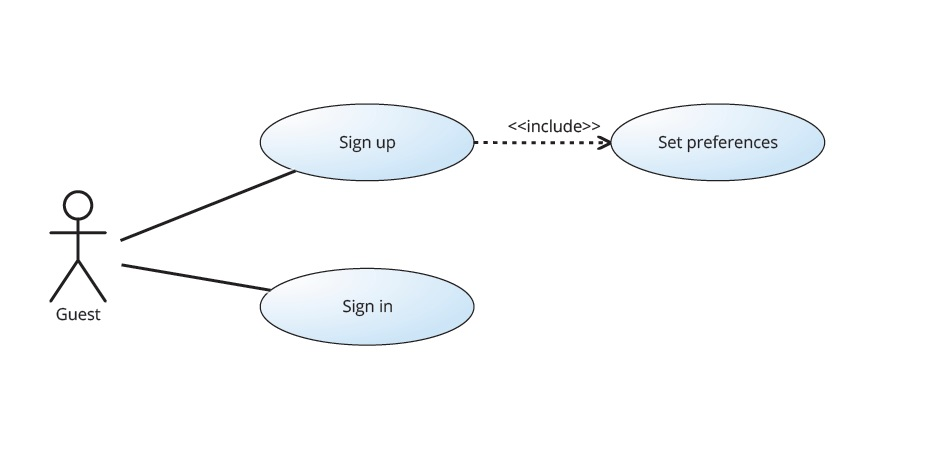
\includegraphics[scale=0.55]{MainMatter/images/usecases/guest}
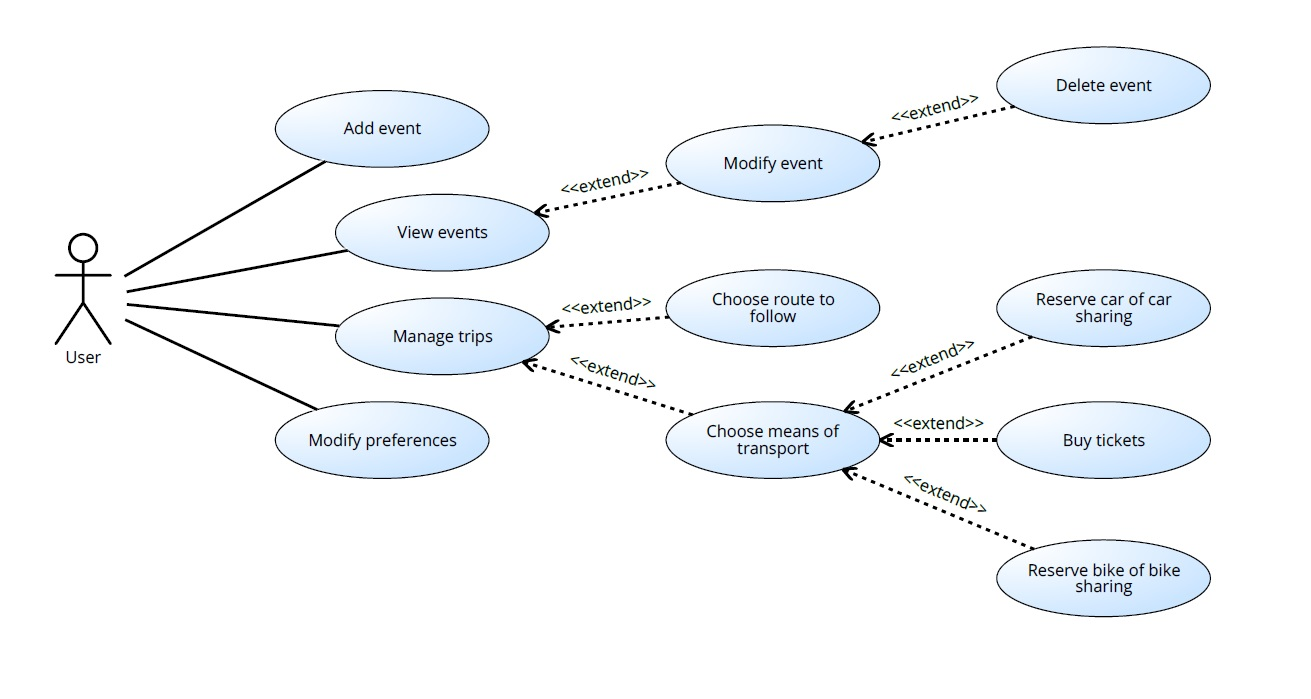
\includegraphics[scale=0.55]{MainMatter/images/usecases/user}
\captionof{figure}{Use case diagram}
\end{center}
\pagebreak
%
\begin{landscape}
\subsection*{Class diagram}
\begin{center}
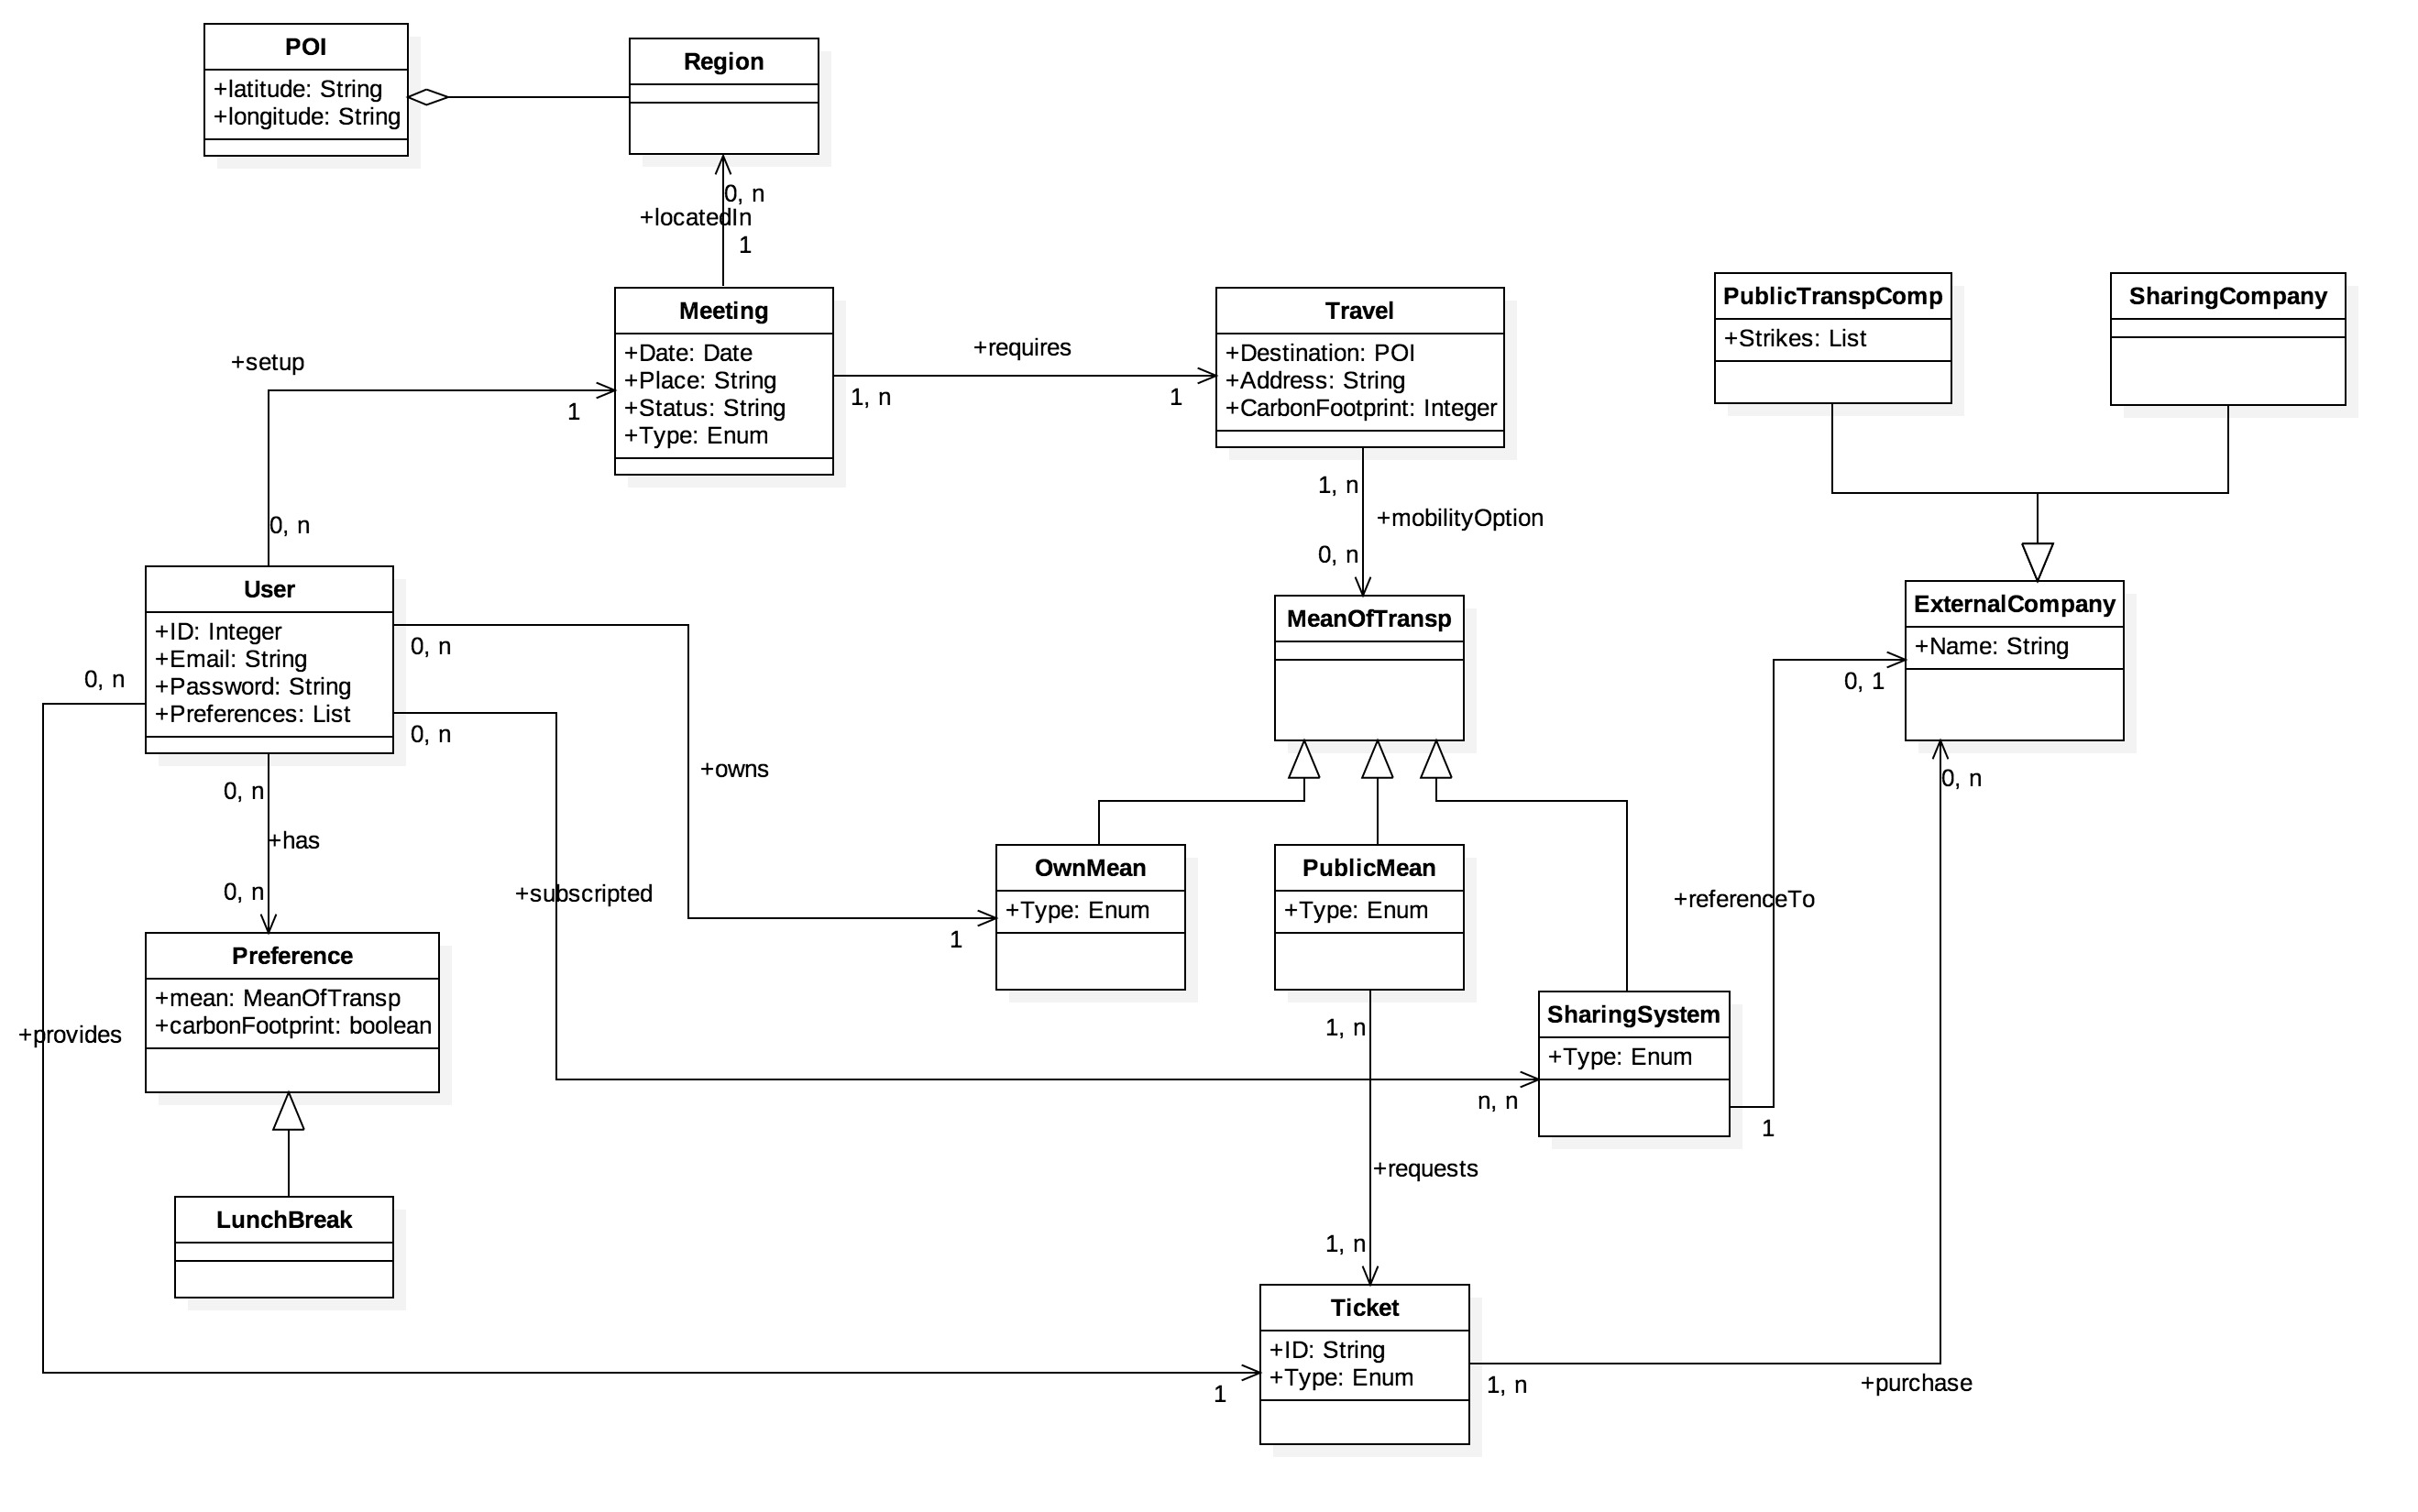
\includegraphics[scale=0.2]{MainMatter/images/uml/uml}
\captionof{figure}{Class diagram of the application}
\end{center}
\end{landscape}
%
% ------------------------------------------------------------------------ %
%
\section{Product Functions}
******************************************************************************************************************************************** \\
Requirements
\\
\\
\subsection*{Scenarios}
In the following tables are present some examples of usage of this application:
%
\begin{center}
\def\arraystretch{1.5}
  \begin{tabular}{ | p{0.9\textwidth} | }
    \hline
    First use of the application \\ \hline
    Giovanni Giorgio is a famous Italian musician, who needs to travel a lot around the big city where he lives. He has many daily appointments, so he wants to optimize his displacements, and, on suggestion of his best friend Francesco, he downloads on his brand-new smartphone the Travlendar+ application. As he opens it he is asked to log in or register to the service, so he proceeds to register filling up the form with his email address and password and to accept the user agreement on personal information. He then gets a warm welcome message, explaining him that only this time a little set up is needed. The following application page opens letting him set up his favourite locations, so he enters his house, workplace and children’s school; than he is asked to set up his break times schedule, thus he chooses that from Monday to Friday between 12.30 AM and 2 PM Travlendar+ will keep half an hour free from trips for him to have lunch; next he can customize the time of the day after which using the bike or walking will not be considered anymore by the application, and he chooses 8 PM. He is also asked if he desire to log into his Google account to synchronize the calendar and maps, and he is glad to do that. After he can select his means of travel: he has a car, uses train and frequently gets public transports to move in the city centre, therefore he inserts his season pass; at last he set up to 1,5 km the maximum distance he is willing to walk. Done all of that he notices that he received an email from the Travlendar+ staff asking to click a link to confirm his email, so he does that and begins to use the application. \\ \hline
  \end{tabular}
\end{center}
%
\begin{center}
\def\arraystretch{1.5}
  \begin{tabular}{ | p{0.9\textwidth} | }
    \hline
    Standard usage (default options, notification, map consultation) \\ \hline
    For everyday he needs to go to work in his recording studio, he opens the newly acquired application to set up this event. He goes there from Monday to Friday, beginning at 8 AM and finishing at 12.30 AM so he sets it as a daily recurrent event, excluding Saturday and Sunday, he adds the timetables and chooses location from the favourites. The next day, while he is having breakfast at 7.13 AM, his smartphone beeps in a welcoming way, showing a notice from Travlendar+ that he needs to leave his house in half an hour to reach his workplace in time using the public transports. Thus, he opens the application clicking on the notification and he is presented the trip details screen, showing him on the map the road he needs to take to catch the bus to go to work and that the displacement will take an ETA of 12 minutes in total, from 7.43 AM to 7.55 AM. Giovanni Giorgio, happy to see his new application working as intended - if not, better - leaves his house at the suggested time and gets to work on time. To get home after work hours Travlendar+ suggests that he goes again by public transportation, knowing he didn’t bring his car to work. \\ \hline
  \end{tabular}
\end{center}
%
\begin{center}
\def\arraystretch{1.5}
  \begin{tabular}{ | p{0.9\textwidth} | }
    \hline
    Minimize carbon footprint \\ \hline
    Some days later our Giovanni Giorgio in his free time is exploring the Travlendar+ application, so he presses on the travels button on the main screen and the calendar view transforms, making his events more transparent. Now, before and after his appointments, the trips appeared on the calendar, showing their timetables and an indication of the suggested means of transport. Gazed in curiosity, he presses on the trip to the dentist he added some time before, which says he should go to the by car. The expanded screen containing the path on the map and trip details - labelled as fastest - opens with a soft animation. On the bottom he sees a modify button under the trip details, he presses it and three options show up: fastest, eco-friendly and customized. So, he decides to try an eco-friendly solution because he is not in a hurry and his dentist in not so far away from his house. Therefore, the application suggests going there by foot showing him a new path crossing the park and he gladly keep it as it is now. \\ \hline
  \end{tabular}
\end{center}
%
\begin{center}
\def\arraystretch{1.5}
  \begin{tabular}{ | p{0.9\textwidth} | }
    \hline
    Passengers \\ \hline
    Sometimes Giovanni Giorgio's wife needs his to go take the children at school, so he creates the event and then he selects the forward trip and changes the passengers’ indicator from the default one to three. In this way Travlendar+ will know that he is going by car or by public transportation. The children will have a nice trip this time too! \\ \hline
  \end{tabular}
\end{center}
%
\begin{center}
\def\arraystretch{1.5}
  \begin{tabular}{ | p{0.9\textwidth} | }
    \hline
    Usage of sharing service \\ \hline
    Giovanni Giorgio come to know about an innovative bike sharing service in his city and decides to try it. After enrolling using the dedicated application of the service, he opens Travlendar+ and in the settings, he adds the sharing service to his means of transport selecting it from a list. The other application opens, asking his permission to give information to Travlendar+; he accepts and goes back to Travlendar+, which will now suggest bike trips locating the nearest bike of the sharing service and use this information to calculate the estimated time of leaving from home. \\ \hline
  \end{tabular}
\end{center}
%
\begin{center}
\def\arraystretch{1.5}
  \begin{tabular}{ | p{0.9\textwidth} | }
    \hline
    External event causing exception and consequent hand customized trip \\ \hline
    On an unlucky day Giovanni Giorgio is going to have dinner with some friends and colleagues of the music industry in the city centre, so Travlendar+ suggests him to take his car (obviously not by bike because it is past 8PM). Unexpectedly his car breaks down halfway, so he grabs his smartphone to quickly open the trip and go to the customized option. It opens a menu letting him choose which means of transport he prefers instead of the car; he selects public transport and the application immediately updates the trip using his position. In the end he gets to his dinner on time using the bus, not losing his fame of being a timely man.  \\ \hline
  \end{tabular}
\end{center}

%
\begin{center}
\def\arraystretch{1.5}
  \begin{tabular}{ | p{0.9\textwidth} | }
    \hline
    Lunch break and external trip-changing factors \\ \hline
    On a rainy day Giovanni Giorgio is full of appointments: he must go to work until 12.30 AM and at 2 PM his fans wait for him at a store to have some copies of his last EP signed. He will not be suggested going home to have lunch because there is not enough time to travel back and eat, additionally to the next appointment trip time. Travlendar+ knows it is not suitable to go by bike when it’s raining, thus it suggests him to go by car. However, 20 minutes before he leaves Travlendar+ sends him another notification that due to the intense traffic, he should instead leave in twelve minutes taking the subway to get to work in time. Happy of the close call, Giovanni Giorgio arrives at work on time thanks to Travlendar+. After work the application suggests him to leave immediately for his next appointment location because rain stopped but the weather is going to worsen in an hour; then he will have time to eat from 1.30 PM to 2 PM. Obviously the application knows that until he does not come back home he cannot begin a trip with a personal means of transport, will not suggest going to the next event by car unless he come by car to an appointment. Our man follows the instructions, and everything goes as planned; by now he is in love with his Travlendar+ application.  \\ \hline
  \end{tabular}
\end{center}
%
\begin{center}
\def\arraystretch{1.5}
  \begin{tabular}{ | p{0.9\textwidth} | }
    \hline
    Buy ticket \\ \hline
    Our artist needs to go in a county town near his city to see a house he wants to buy, so he trusts Travlendar+ to arrange the trip for him. The application suggests using the train and the trip screen contains a button indicating the possibility of buying the ticket. He presses it and the application opens a built-in browser that redirects to the train company page selling tickets, so he proceeds buying the ticket with his credit card. The browser closes, and the check-out screen compares. Everything is ready for the trip! \\ \hline
  \end{tabular}
\end{center}
\pagebreak
% ------------------------------------------------------------------------ %
%
\section{User Characteristics}
The user of the system-to-be is every person who wants to schedule appointments in a calendar and manage his movements from a location to another at the same time.
Users can use it to organize work events, but also include family or spare time events. The application doesn't have any age limit, or any other restriction applied to the user characteristic. In order to make the application work without limitation the user need to have access to the Internet, but he can access and modify the calendar offline.
%
% ------------------------------------------------------------------------ %
%
\section{Assumptions, Dependencies, Constraints}
**************************************************************************************************************************************************************************** \\
Domain assumptions
\\
\\
Regulatory policy:
The System asks the User for the permission to acquire, store and use his personal data, and informs him that won't take any responsibility for a use of it that doesn't complies with the local laws and policies, by means of the User agreement's acceptance.
The System under request of the User must delete all his personal data.
%
% -----------------------------END------------------------------------- %